\chapter{Hazard analysis dell'Apparato IMR}

In questo capitolo viene riportata l'analisi dei rischi vera e propria. Sono state studiate tutte le situazioni pericolose e i rischi associati e sono state individuate mitigazioni per permettere di ridurre la probabilit� di occorrenza degli hazards a un livello accettabile, aumentando la safety del sistema. Come suggerito dalla tecnica HAZOP, il sistema viene suddiviso in pi� parti e per ognuna di esse viene innanzitutto definito l'intento progettuale.\\
In seguito, vengono selezionati gli elementi delle parti e per ognuno di essi vengono applicate le parole guida elencate nei capitoli precedenti in ogni loro interpretazione. Se tale procedura evidenzia delle criticit�, verranno indagate le rispettive cause e conseguenze.\\
Per ogni rischio evidenziato verranno riportati la frequenza di occorrenza e la severit� dell'azzardo; dall'unione di queste due informazioni verr� ricavata la valutazione dell'azzardo in questione. Se il livello di rischio � trascurabile o tollerabile non sar� necessario individuare la mitigazione. Al contrario, se il livello del rischio � indesiderabile o intollerabile, verr� riportato un appropriato meccanismo di protezione o delle indicazioni atte a risolvere la problematica rilevata.\\Una volta che verranno applicate le interpretazioni di tutte le parole guida a tutti gli elementi progettuali, la sezione sar� contrassegnata come completata e si passer� ad esaminare le parti successive.\\ Tutte le informazioni relative all'Hazard analysis sono riportate in un file Excel con lo scopo di tener traccia di tutte le cause, conseguenze e mitigazioni rilevate. In tale file excel ogni azzardo viene contrassegnato in maniera univoca da un id in modo tale da riuscire a orientarsi nella tabella.\\

\section{Schema funzionale}

Per riuscire a comprendere a pieno tutti i compiti e le operazioni che devono essere effettuate dai componenti presenti nell'apparato IMR � stato necessario utilizzare uno schema funzionale. Tale schema descrive graficamente tutti gli attori del sistema e i rispettivi ruoli: in verde sono riportati i componenti, in rosso i blocchi che descrivono operazioni critiche e in blu i blocchi che descrivono operazioni non critiche. 
\begin{figure}[htbp]
	\centering
	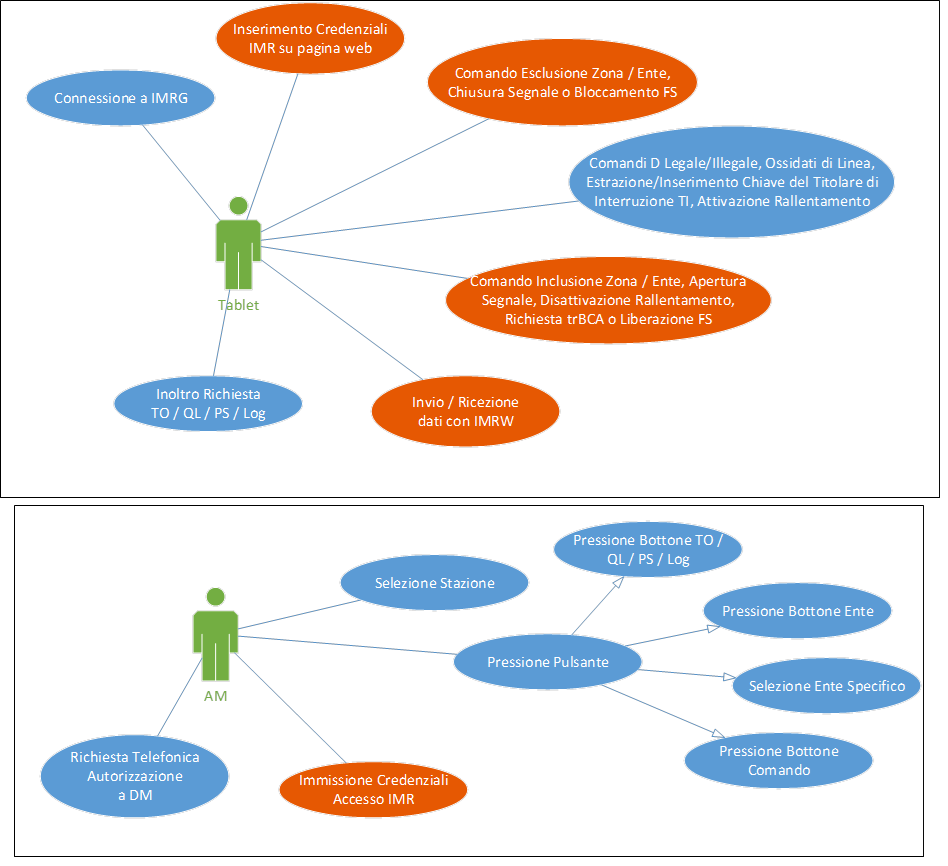
\includegraphics[scale=0.6]{img/schematablet}
	\caption{Schema funzionale Tablet Operatore e AM}
\end{figure}
\begin{figure}[htbp]
	\centering
	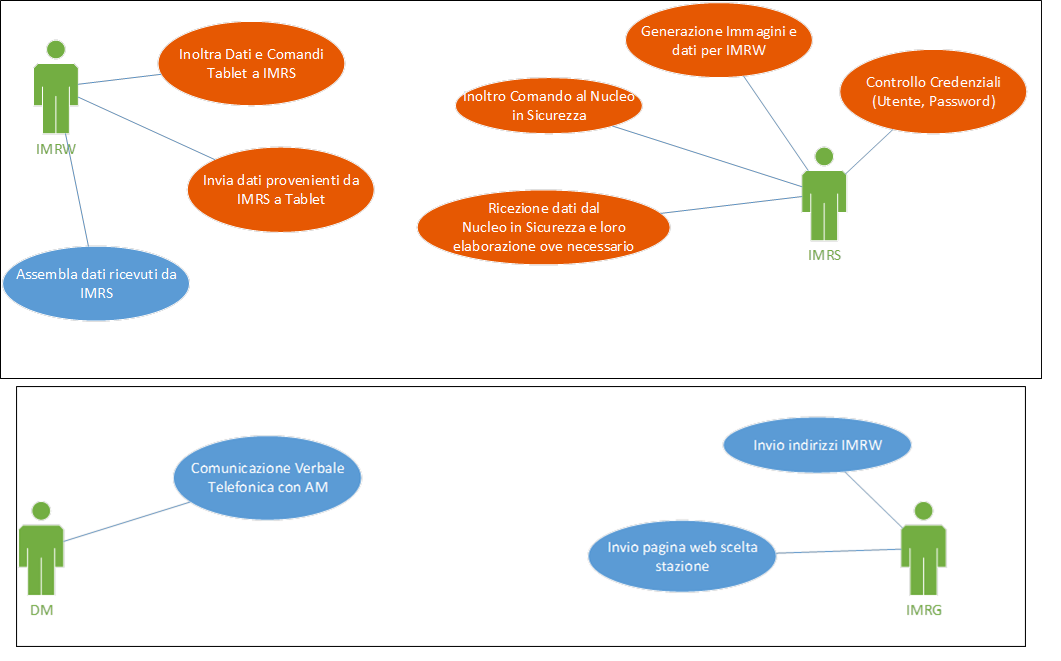
\includegraphics[scale=0.6]{img/schemaimrw}
	\caption{Schema funzionale IMRW, IMRS, DM e IMRG}
\end{figure}
\newline
\newline
\newline
\newline
\newline

\section{Autenticazione Tablet e Scelta Stazione}

La prima parte del sistema analizzata � quella relativa all'autenticazione sul Tablet e alla selezione della stazione d'interesse da parte dell'addetto manutenzione (AM).\\
Durante questa fase i componenti attivi sono: 
\begin{itemize}
	\item Addetto manutenzione;
	\item Tablet;
	\item Server IMRG;
	\item Server IRMW.
\end{itemize}
\begin{figure}
	\centering
	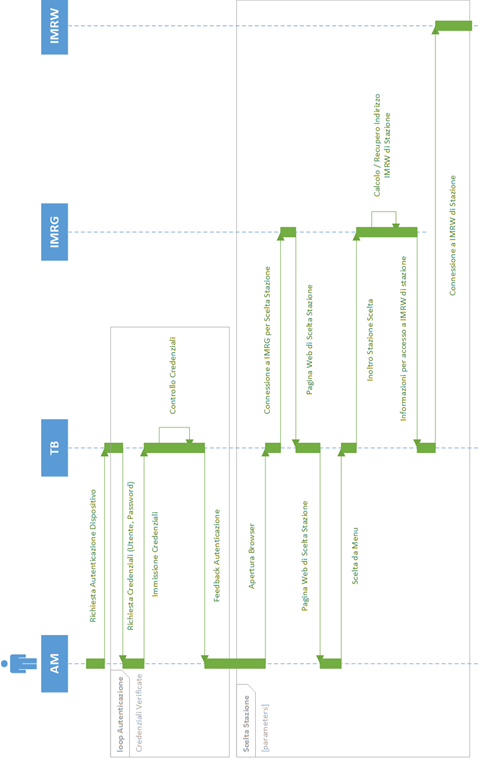
\includegraphics[scale=0.7]{img/sdprimo}
	\caption{Sequence Diagram prima fase}
\end{figure}
Come viene evidenziato dal sequence diagram questa sezione pu� essere divisa in due sottosezioni:
\begin{itemize}
	\item loop autenticazione;
	\item scelta stazione.
\end{itemize}
L'autenticazione al dispositivo � la prima operazione che l'addetto manutenzione deve effettuare, durante questa fase le credenziali vengono verificate direttamente dal Tablet.
Il server IRMG sar� presente solo in questa fase e nella successiva, in quanto il suo unico ruolo � quello di reindirizzare la connessione verso il server IRM locale e di memorizzare le chiavi pubbliche dell'AM. La reindirizzazione all'IMRW avviene immediatamente dopo la scelta della stazione da parte dell'addetto manutenzione.

\subsection{Rischi individuati}

Durante l'analisi di questa fase sono stati individuati vari rischi mediante l'utilizzo delle parole guida viste in precedenza. Tale analisi ha evidenziato quasi tutti rischi \textit{tollerabili}, infatti molto spesso la severit� di suddetti rischi � stata classificata come \textit{insignificante}, in quanto gli azzardi non comportano problemi per la safety. \\ 
\begin{figure}[htbp]
	\centering
	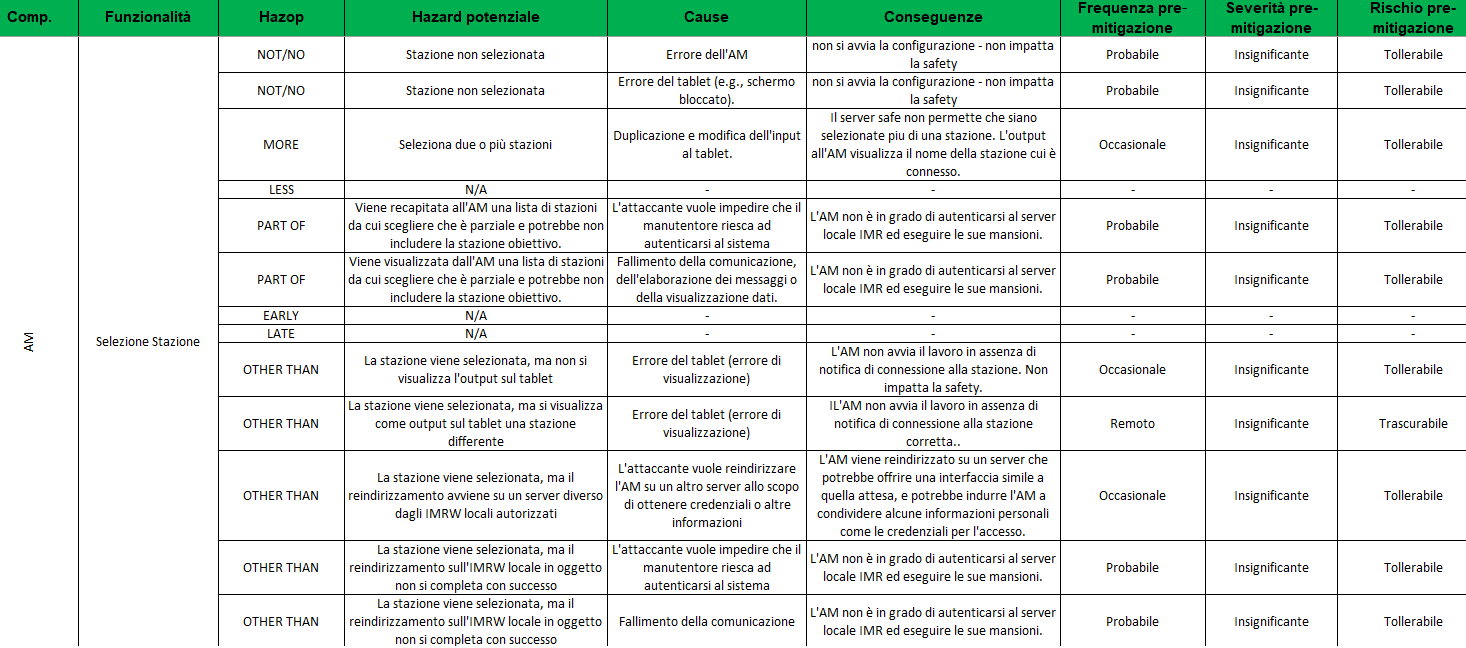
\includegraphics[scale=0.5]{img/exceluno}
	\caption{Esempio hazard analysis prima fase}
\end{figure}

\section{Login IMR}

\begin{figure}
	\centering
	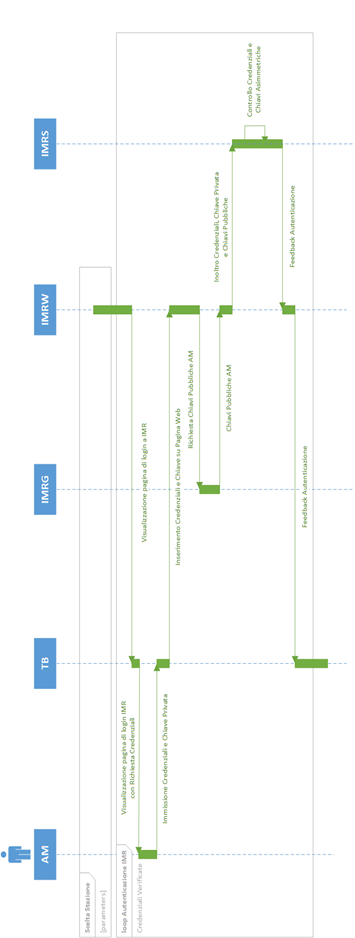
\includegraphics[scale=0.7]{img/sdsecondo}
	\caption{Sequence diagram seconda fase}
\end{figure}

Nella fase di autenticazione intervengono: 
\begin{itemize}
	\item Addetto manutenzione;
	\item Tablet;
	\item Server IMRG;
	\item Server IRMW;
	\item Server IMRS.
\end{itemize}
L'operazione di autenticazione coinvolge praticamente tutti i componenti dell'apparato IMR. Questa operazione avviene mediante ID/Password e un meccanismo di chiave asimmetrica (pubblica-privata). L'addetto manutenzione immette le proprie credenziali e la chiave privata, la chiave pubblica � invece memorizzata dal server centrale IMRG che ha il compito di inviarla all'IMRW. Il server IMRW inoltra tutte le informazioni relative all'autenticazione al server IMRS che si occuper� di verificare l'effettiva correttezza di quest'ultime e quindi di inviare la schermata del Terminale Operatore al Tablet se l'utente � autorizzato. IMRS � un server sicuro, progettato, sviluppato e certificato SIL4 ed � per questo che il controllo delle credenziali viene effettuato su quest'ultimo e non su IMRW.

\subsection{Rischi seconda parte}


\section{Visualizzazione Terminale Operatore (TO)}

\begin{figure}
	\centering
	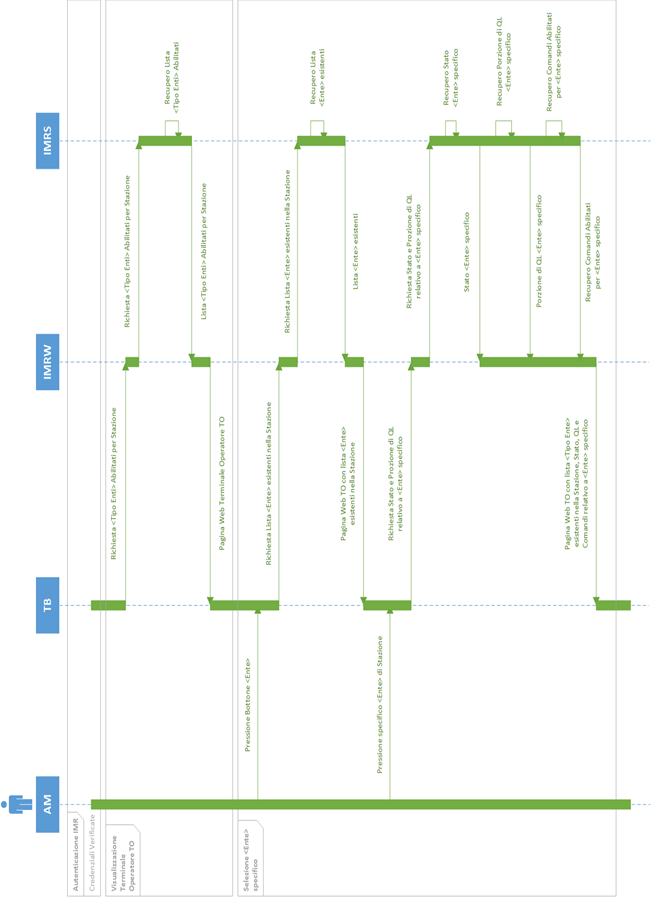
\includegraphics[scale=0.7]{img/sdterzo}
	\caption{Sequence diagram terza fase}
\end{figure}

Durante le operazioni relative a questa fase possiamo individuare: 
\begin{itemize}
	\item Addetto manutenzione;
	\item Tablet;
	\item Server IRMW;
	\item Server IMRS.
\end{itemize}

Anche qui, � possibile rilevare due sottosezioni:
\begin{itemize}
	\item visualizzazione Terminale Operatore TO;
	\item selezione <Ente> specifico.
\end{itemize}
Infatti, dopo aver verificato la correttezza delle credenziali, viene inviata dall'IMRS al Tablet la pagina web del Terminale Operatore che riporta tutti gli Enti abilitati per quella determinata stazione.\\ L'addetto manutenzione pu� quindi iniziare a inviare i comandi opportuni per le operazioni di manutenzione. L'AM in questa fase � infatti in grado di premere i bottoni degli <Enti> di stazione e l'IMRS inoltrer� la relativa pagina Web TO con lista <Tipo Ente> esistenti nella Stazione, Stato, QL, e i comandi relativi all'Ente specifico.


\subsection{Rischi terza parte}


\section{Esecuzione comando AM}

NON VA BENE IL SEQUENCE DIAGRAM

\section{Selezione Piano Schematico (PS), Quadro Luminoso (QL), Log}
